% Chapter Template

\chapter{Network Components and Protocols} % Main chapter title

\label{Chapter3} % Change X to a consecutive number; for referencing this chapter elsewhere, use \ref{ChapterX}

\lhead{Chapter 3. \emph{Network Components and Protocols}} % Change X to a consecutive number; this is for the header on each page - perhaps a shortened title

%----------------------------------------------------------------------------------------
%	SECTION 1
%----------------------------------------------------------------------------------------

\section{802.1X}



\section{RADIUS}


\section{WiSM}



\section{DHCP}



\section{SNMP}
The Simple Network Management Protocol is an application layer protocol that facilitates the exchange of management information between network devices \cite{snmp}. It is part of the TCP/IP protocol suite and it is mainly used by network administrators to get information about devices on the network and the network performances. These information help the administrators to resolve problems on the network or simply to manage it.\\
A SNMP network has three main components:
\begin{itemize}
	\item \texttt{Network-management system (NMS)}: A NMS is the main component of an SNMP-managed network. It is the management entity that controls the managed devices. It uses the SNMP protocol and can interact with the managed devices to get information using special commands and messages.
	
	\item \texttt{Managed devices}: It is a network device that contains an SNMP agent. They collect and store information to make them available for the network-management systems. Those devices can be routers, servers, switches,etc. They also run the SNMP protocols to be able to respond to the requests made by the NMS.
	
	\item \texttt{Agents}: An agent is the thinking part of a managed device. It is a software module that understands the management information and translates them into a SNMP compatible form.
\end{itemize}
Here is a figure showing a SNMP-managed network.
\begin{figure}[H]
	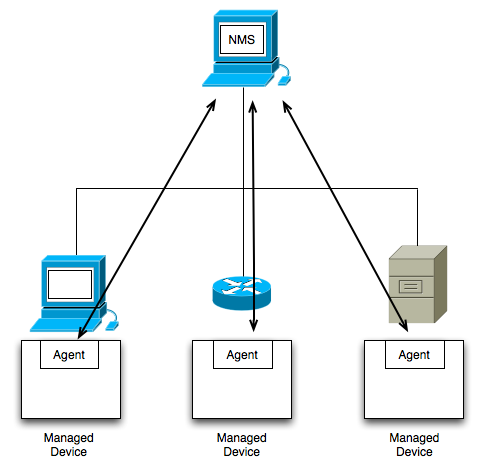
\includegraphics[width=.7\linewidth]{Pictures/Chapter3/snmp.png}
\end{figure}

All the network objects are described and organized hierarchically in a Management Information Base (MIB). There are MIBs for each set of related network entites that can be managed. These MIBs are accessed using a network-management protocol such as SNMP.


\section{Problems encountered}